\documentclass{article}
\usepackage{changepage}
\usepackage{float}
\usepackage{amsmath}
\usepackage{tikz}
\usepackage{graphicx}
\usepackage{color}
\usepackage{listings}

\definecolor{dkgreen}{rgb}{0,0.6,0}
\definecolor{gray}{rgb}{0.5,0.5,0.5}
\definecolor{mauve}{rgb}{0.58,0,0.82}

\lstset{frame=tb,
  language=Java,
  aboveskip=3mm,
  belowskip=3mm,
  showstringspaces=false,
  columns=flexible,
  basicstyle={\small\ttfamily},
  numbers=none,
  numberstyle=\tiny\color{gray},
  keywordstyle=\color{blue},
  commentstyle=\color{dkgreen},
  stringstyle=\color{mauve},
  breaklines=true,
  breakatwhitespace=true,
  tabsize=3
}
\begin{document}
\noindent
\begin{center}
Andreas Landgrebe
\\
Computer Science 250: Analysis of Algorithms
\\
Laboratory Assignment 2
\\
Experimental Verification of Runtimes

\end{center}

\newpage
\begin{center}
\Huge Part 1 
\end{center}
\begin{figure}[H]
\centering
\begin{adjustwidth}{-3cm}{}
\begin{tabular}{| l | l | l | l | l | l | l | l |}
\hline
FourSum.java & Run 1 & Run 2 & Run 3 & Run 4 & Run 5 & Mean(Average) & Standard Deviation \\ \hline
1Kints & 81.454 & 82.408 & 81.513 & 81.407 & 81.341 & 81.62646 & 0.39574662212515 \\ \hline
2Kints & 1298.131 & 1298.078 & 1298.968 & 1298.089 & 1298.506 & 1298.3544 & 0.34531990964905 
\\ \hline
4Kints & 20,759.469 & 20,733.701 & 20,729.643 & 20,724.63 & 20,730.529 & 20,735.5944 & 12.287204687805
\\ \hline

\end{tabular}
\caption{Table of Results of Part 1 of Laboratory Assignment (seconds)}
\end{adjustwidth}
\end{figure}

2. Determine the runtime of this algorithm in Big-O notation, and estimate what you would expect to find using tilde notation (a detailed calculation is not necessary for this step).
\\
Big-O Notation = $O(n^4)$
\\
Tilde Notation/ Tilde Approximation: $~ \frac{n^4}{24}  $
\\
\\
4. How long do you expect execution will take on the 2Kints.text file? Note this somewhere, as I will ask for it later. 
\\
Since 1Kints took 80 seconds, I estimate 2Kints to take 1280 seconds long
\\
\\
6. How long do you expect execution will take on the 4Kints.txt file?
\\
4Kints estimated time: 20480 seconds
\\
\\
8. Is a pattern becoming apparent? How long do you expect execution will take on the 8Kints.txt file? The 16Kints.txt file? The 1Mints.txt file?
\\
8Kints estimated time: 327680 seconds
\\
16Kints estimated time: 5242880 seconds
\\
1Mints estimated time: $ 8 * 10^{13}$ seconds
\\
\\
11. Create two graphs, a linear-axis graph and a log-log axis graph, showing how your mean program runtimes increased as input size increased. 
\\
\newpage
\begin{center}
Linear Axis Graph of Part 1
\end{center}
\begin{center}
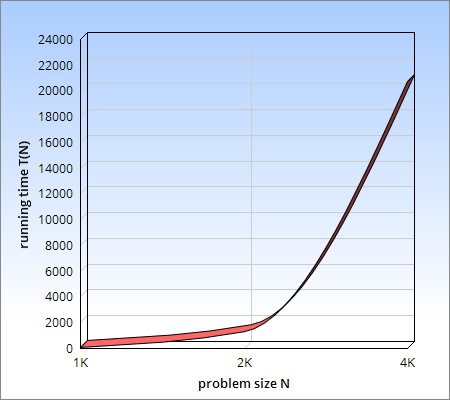
\includegraphics[width=6.45cm]{Part1Linear.png}
\end{center}
%might need to add something more later for the questions that are asked in Part 1
\begin{center}
Log-Log axis graph of Part 1
\end{center}
\begin{center}
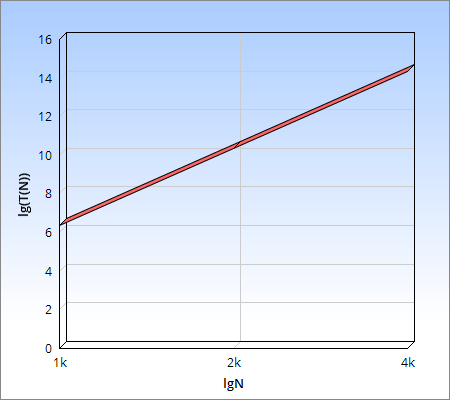
\includegraphics[width=6.45cm]{Part1Log.png}
\end{center}
\newpage
\begin{center}
\Huge Part 2
\end{center}
\begin{figure}[H]
\begin{adjustwidth}{-3cm}{}
\begin{tabular}{| l | l | l | l | l | l | l | l |}
\hline
FourSumFast.java & Run 1 & Run 2 & Run 3 & Run 4 & Run 5 & Mean(Average) & Standard Deviation \\ \hline
1Kints & 5.177 & 5.149 & 5.157 & 5.154 & 5.146 & 5.1566 & 0.010892199043352 
\\ \hline

2Kints & 45.241 & 45.511 & 44.476 & 45.496 & 44.997 & 45.1442 & 0.38362346122207
\\ \hline

4Kints & 388.047 & 386.84 & 387.791 & 391.895 & 387.39 & 388.3926 & 1.7979956173473
\\ \hline

8Kints & 3271.271 & 3294.607 & 3307.508 & 3288.185 & 3295.925 & 3291.4992 & 11.880166672231
\\ \hline
\end{tabular}
\caption{Table of Results of Part 2 of Laboratory Assignment (seconds)}
\end{adjustwidth}
\end{figure}
2. Determine the runtime of this algorithm in Big-O notation.
\\
Big-O notation: $O(n^3 (\log (n))$
\\
3. How long do you expect execution will take on the 1Kints.txt file, knowing the performance that you measured with FourSum?
\\
Knowing the performance of 1Kints on FourSum, I expect the execution to be 5 seconds.
\\
\\
5. How long do you expect execution will take on the 2Kints.txt file?
\\
I expect the execution time on the 2Kints.txt file to be 50 seconds.
\\
\\
7. How long do you expect execution will take on the 4Kints.txt file?
\\
I expect the execution time will take 320 seconds on the 4Kints.txt file
\\
\\
9. You should once against see the pattern emerge. How long do you expect execution will take on the 8Kints.txt file? The 16Kints.txt file? The 1Mints.txt file?
\\
8Kints : 2560 seconds
\\
16Kints : 20480 seconds
\\
1Mints : $2.982894 * 10^{10}$
\\
\newpage
\begin{center}
Linear Axis Graph of Part 2
\end{center}
\begin{center}
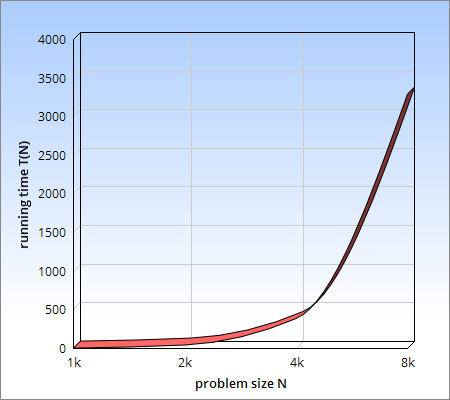
\includegraphics[width=6.45cm]{Part2Linear.png}
\end{center}
\begin{center}
Log-Log axis graph of Part 2
\end{center}
\begin{center}
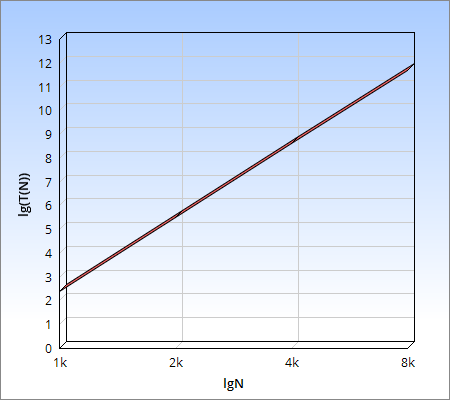
\includegraphics[width=6.45cm]{Part2Log.png}
\end{center}
\newpage
\begin{center}
\Huge Part 3
\\
\Huge While You Have Some Downtime 

\end{center}
\begin{enumerate}
\item Consider the following code segment. Calculate its approximate runtime, in both tilde notation and in Big-O notation.
\\
\begin{lstlisting}
int sum = 0;
for (int i = 1; i < n; i *= 2) {
	for (int j = 0; j < n;  j++) {
		sum++;
	}//for
}//for
\end{lstlisting}
Big-O Notation: $O(n log (n))$
\\
Tilde Notation: $2n log(n) $

\item Sketch an algorithm that, given two sorted arrays of $n$ int values, prints all elements that appear in both arrays, in sorted order. Show that the running time of your algorithm is $O(n)$ in the worst case.
\\
\begin{lstlisting}
int [] a; //declaring the array a
int [] b; //declaring the array b
int [] c = new int[Math.min(a.length, b.length)];
int a1 = 0;
int b1 = 0;
int c1 = 0;
while (a1 < a.length && b1 < b.length) {
	if(a[a1] < b[b1]) {
		a1++;
	} else if (a[a1]  > b[b1]) {
		b1++;
	}else {
		if (c1 == 0 || a[a1] != c[c1 - 1]) {
				c[c1++] = a[a1];
			}
		a1++; b1++;
		}
	}
	return Array.copyOfRange(c, 0, c1);
}

\item What does the following recursive function return
\begin{lstlisting}
public static String mystery(String s){
	if (s.length() <= 1) {
		return s;
	}else {
		String a = a.subString(0, s.length()/2);
		String b = b.subString(s.length()/2, s.length());
		return mystery(b) + mystery(a);
	}//if-else
}//mystery
\end{lstlisting}
This recursive function will return a string in reverse order.
\item How much physical memory was taken up by the contents of the 1Kints.txt file when loaded into a one-dimensional array? The 2Kints.txt file? 4Kints.txt? 1Mints.txt? How much physical memory would be taken up if the files contained doubles rather than int? How much physical memory would be taken up if each of the file inputs were arranged in a two-dimensional array with 100 rows (1000 ints in a 100x10 array, 200 ints in a 100x20 array, etc.)? (Note: I am looking for exact numbers of bytes here, not an approximation based off of tilde notation.)
\\
\textbf{Ints}
1Kints.txt file in one-dimensional array: 1,024 bytes
\\
2Kints.txt file in one-dimensional array: 8,024 bytes
\\
4Kints.txt file in one-dimensional array: 16,024 bytes
\\
1Mints.txt file in one-dimensional array: 4,000,024 bytes
\\
If the files contained doubles instead rather than ints, then an array of n doubles would be 24 + 8n, so:
\\
\textbf{Doubles}
\\
1K file in one-dimensional array: 8,024 bytes
\\
2K file in one-dimensional array: 16,024 bytes
\\
4K file in one-dimensional array: 32,024 bytes
\\
1M file in one-dimensional array: 8,000,024 bytes
\\
Two Dimensional Array: 
\\
1000 ints in a 100 x 10 array: 4000 bytes
\\
200 ints in a 100 x 20 array: 8000 bytes
%answer goes here
\item As a review of working with the Stack data structure, create a file called Parantheses.java that reads in text from standard input and uses a stack to determine whether its parantheses are properly blanced. For example, your program should print true for [()]\{\}\{[()()]()\} and false for [(]).
\begin{lstlisting}
import java.util.*;
import java.io.*;


public class Parentheses {
    private static final char L_PAREN    = '('; //this is the declaration for the left parantheses (
    private static final char R_PAREN    = ')'; //this is the declaration for the right parantheses )
    private static final char L_BRACE    = '{'; //this is the declaration for the left brace {
    private static final char R_BRACE    = '}'; //this is the declaration for the right brace }
    private static final char L_BRACKET  = '['; //this is the declaration for the left bracket )
    private static final char R_BRACKET  = ']'; //this is the declaration for the right bracket )

    public static boolean isBalanced(String s) {
        Stack<Character> stack = new Stack<Character>(); //declartion of a stack
        for (int i = 0; i < s.length(); i++) {

            if      (s.charAt(i) == L_PAREN)   stack.push(L_PAREN); //if a left parantheses is found, then push it to the top of the stack

            else if (s.charAt(i) == L_BRACE)   stack.push(L_BRACE); //if a left brace is found, then push it to the top of the stack

            else if (s.charAt(i) == L_BRACKET) stack.push(L_BRACKET); //if a left bracket is found, then push it to the top of the stack

            else if (s.charAt(i) == R_PAREN) {
                if (stack.isEmpty())        return false;
                if (stack.pop() != L_PAREN) return false;
                //is the right parantheses and left parntheses cannot be matched, then return false
            } //if

            else if (s.charAt(i) == R_BRACE) {
                if (stack.isEmpty())        return false;
                if (stack.pop() != L_BRACE) return false;
                //if a right brace cannot be matched with a left brace, then return false
            } //if

            else if (s.charAt(i) == R_BRACKET) {
                if (stack.isEmpty())        return false;
                if (stack.pop() != L_BRACKET) return false;
                //if a right bracket and left bracket cannot be matched, then return false. 
            } //if

            // ignore all other characters

        } //for
        return stack.isEmpty(); 
    } //isBalanced


    public static void main(String[] args) {
        String s = StdIn.readAll();
        System.out.println(isBalanced(s)); //print line statement to call the method isBalanced with a string as a parameter
    } //main

} //Parantheses.java
\end{lstlisting}
\end{enumerate}





\end{document}